To measure influence in the newspaper environment and to compare and rank people as influential, we define an influence score measure called \textit{``Influential Person Index" (IPI)} corresponding to each person entity in the people gazetteer. To calculate IPI for each person entity, we first define the \textit{``Document Index" (DI)} to measure how each document in the person entity's associated list of documents affects his influence score.
The choice of features for detecting a person entity as influential is motivated by following questions: Are frequently occurring persons in the newspaper influential? Does frequency mean occurrences of a person entity in a single article or across complete dataset? Do longer documents tend to talk about more important persons? Is a person entity occurring over multiple topics more influential or the one who is consistently talked about in similar topic articles? 

Following subsections describe the features/parameters chosen for calculation of DI and IPI of a person entity followed by the complete algorithm for detection of influential persons:

\subsection{Document Index (DI)}
\label{influential:DI}
The Document Index (DI) of an article in the people gazetteer helps to measure a person's influence score. Following parameters are considered for the calculation of this index:

\begin{enumerate}
\item \textbf{Normalized Document Length} (NDL)\\
Document Length affects the influence score in the sense that a longer news article in which a person entity occurs is deemed to be more important than a shorter one. It is defined as the number of tokens contained in a news article. Document Length is further normalized by dividing it with the maximum news article length (of 14020 articles in the dataset) to get Normalized Document Length as follows: 

$$NDL=\dfrac{\text{Document Length}} {\text{Maximum Document Length in the dataset}}$$


%\item[$\bullet$IDF]
%IDF is used as a parameter in the calculation of DI of a news article to give weight to the person entity's occurrence in the complete %dataset. It can be calculated as the number of news articles in which a person entity occurs in the complete dataset. It is %equivalent to the length of document list in the people gazetteer for each person entity.

\item\textbf{ Normalized Term Frequency} (NTF)\\
Term Frequency (TF) accounts for the number of occurrences of a person's name in a news article. The TF of the person name affects a document's influence score as a higher number of occurrences in the document makes it more important. TF is further normalized and calculated as follows:

\begin{center}
$NTF=	1	+\log	$(TF of person entity in current article)
\end{center}


The issues of co-reference resolution of person names (For Example, person entities such as ``William Schmittberger",``Captain Williams" are same but recognized as separate persons) and named entity disambiguation ( Occurrence of different persons with similar name in news articles. For example, the person ``John Smith" detected in two different articles might or might not be the same person) occur in our People Gazetteer which are not taken care of by PNER and need to be addressed separately. While the issue of co-reference can be still addressed by analyzing each news article, it is extremely hard to disambiguate among persons with similar names that can occur in multiple news articles with different topics. This is the reason coreference resolution is performed for the person entities obtained using PNER.The following section explains the approach to coreference resolution followed after development of People Gazetteer.


\subsubsection{Coreference Resolution}
 The coreference resolution aims to find out all expressions that refer to the same entity in the text. Due to multiple references to a person in the text,coreference resolution been done keeping in mind that the number of articles of occurrence of a person entity, i.e.,TF is an important parameter in our study for determining an influential person.

Coreference resolution is performed using the Standford Deterministic Coreference Resolution System of the Stanford CoreNLP toolkit /footnote{http://nlp.stanford.edu/software/dcoref.shtml}. It uses a multi-pass seive coreference resolution\cite{lee2013deterministic} which consists of 3 steps: mention detection which identifies clusters of all noun phrases, pronouns and named entity mentions, coreference resolution step which is a combination of ten independent seives applied from highest to lowest precision one by one sequentially but with global information sharing so that each seive builds on the previously clustered mentions followed by post processing which removes singleton mentions.
Coreference Resolution was observed to be useful during this case study since the frequency of a person entity in a newspaper article changes when multiple references to the same person entity are found in an article. 


\item \textbf{Number of similar articles} (NSIM)\\
This parameter is used in calculation of the DI by finding articles of similar topic in the document list. 
%The set of topics derived from a corpus can be used to answer questions about the similarity of words and 
%documents.
Two documents are considered similar if they belong to the same topics. For a document $d$ whose DI is to be calculated, we consider 

SIM= Number of articles with the same topic as that of $d$ in the document list of person entity.

This measure is normalized by dividing it with the number of total articles in the document list of the person entity as follows:

\begin{center}
$NSIM= \dfrac{\text{SIM}} {\text{Total number of articles in the person's document list}}$
\end{center}
NSIM can be said to be equivalent to the proportion of topic similar articles that any document $d$ has.

This parameter takes into account the effect of a document's score on a person's IPI when there exist several other documents of the same topic in the person's list. 


\end{enumerate}

DI for each document is a function of the above mentioned parameters and is calculated using the following formula :
\begin{center}

			$DI = w_a . NDL + w_b . NSIM + w_c . NTF $
\end{center}
where, $w_a$,$ w_b$ and $w_c$ are the weights associated with each of the parameters NDL, NSIM and NTF respectively.


DI is actually a heuristic measure of these three parameters where each of the parameters can be weighted as per dataset characteristics and user requirements. For example, a higher value to $w_a$ and lower to $w_b$ and $w_c$ indicates documents with longer lengths are considered more important for influencing a person's IPI. On the other hand, a higher value to $w_b$ and lower to $w_a$ and $w_c$ indicates a document with larger proportion of topic similar articles influences the person's IPI more suggesting assignment of high influence score to a person entity occurring repeatedly in a specific news topic.  

\subsection{Influential Person Index (IPI)}

Once DI is calculated for each document in a person's list, an index is calculated for the person entity in order to measure its influence in the news dataset and calculate its influential score. The ``Influential Person Index" defined for this purpose is calculated as follows:
		
\begin{center}
$IPI= max DI(d_1, d_2, ...,d_n)+ UniqT$
\end{center}

where , $max DI(d_1, d_2, ...,d_n)$ = Maximum Document Index of a document $d_i$ in a person entity's list of  $n$ articles, and
\begin{center} $UniqT = \dfrac{\text{Number of Unique Article Topics in a person entity's document list}}{\text{Total Number of Topics in the corpus}}$\end{center} 

The parameter $UniqT$  is used to account for the fact that a single person entity can be talked about multiple news topics in the news articles and to include its effect on the person entity's influence score. It is normalized by dividing it with the total number of topics as obtained during topic detection on all 14020 articles.

Ranking is done across each person category of the people gazetteer to obtain top most influential persons. For this, IPI for each person entity across the person categories are sorted in decreasing order to obtain the most influential person entities with highest IPI at the top.
  
\subsection{Procedure for finding influential persons}

Algorithm ~\ref{algorithm:3} depicts the procedure for measuring influence and ranking of influential people from the gazetteer. It starts with calculation of DI for each news article in a person's document list by calculating the required parameters of NDL, NSIM and NTF which are assigned 0 values initially. The respective weights $w_a$,$w_b$,$w_c$ are taken as inputs and multiplied with each parameter to get final DI score which is added to the list of DI scores $DIScoreList$. The list is sorted to find the maximum DI value among all news articles in the person's document list. The maximum DI score is then added to the UniqT parameter to get the final IPI for each person entity which are again stored and sorted to obtain a ranked list of influential person entities.  



\begin{algorithm}[!htb]
\caption{Procedure to calculate IPI and rank person entities based on it}
\label{algorithm:3}
\begin{algorithmic}
\Function {CalculateIPI}{}
  

%%%%%%DOUBT HERE.....
 \KwIn{$PeopleGazetter(Persons,(DocList,$}
\KwIn{$TopicList))$, $w_a$,$w_b$,$w_c$}
\KwResult{Ranked list of Person Name and IPI}  
 $NTF \leftarrow $0,  $NDL \leftarrow $0, $NSIM \leftarrow $0, $DI\leftarrow $0, $UniqT\leftarrow $0, $IPI\leftarrow $0\;  
  
    \For{(String PersonName : Persons)}
     {
	   \For{(String doc  : DocList)}
	{	
		$NTF=1+\log (GetPersonTF(doc))$;
		
$NDL=GetDocLength(doc)/GetMaxDocLength()$;

		$ NSIM=GetTopicSimilarArticles(doc,DocList)$;

		$DI=w_a . NDL+w_b . NSIM+ w_c . NTF$;
		
		$DIScoreList.add(DI)$;
 	 }
		$Sort(DIScoreList)$;

		$UniqT=GetUniqueTopics(Person,TopicList)$;

		$IPI=Max(DIScoreList)+UniqT$;

		$IPIScores.put(PersonName,IPI)$;
       }
	$Sort(IPIScores)$;

	$PrintPersonNameandMaxIPI(IPIScores)$;

\EndFunction
\end{algorithmic}
\end{algorithm}

\begin{table*}
\begin{center}
\begin{tabular}{|c|c|} \hline
Function Name & Description \\ \hline
GetPersonTF(doc) & Calculates TF of the person entity \\
 & in document $doc$ \\ \hline
GetDocLength(doc) & Calculates number of tokens in $doc$. \\ \hline
GetMaxDocLength() & Calculates maximum number of \\
& tokens in any document.\\ \hline
GetTopicSimilarArticles(doc,DocList) &  Calculates normalized number \\
& of topic similar articles for $doc$ in the $DocList$. \\ \hline
Sort(DIScoreList) & Sorts the $DIScoreList$ \\ \hline
Max(DIScoreList) & Finds the maximum score from $DIScoreList$. \\ \hline
GetUniqueTopics(Person,TopicList) & Calculates normalized unique \\
& topics for $Person$ in its $TopicList$. \\ \hline
Sort(IPIScores) & Sorts the $IPIScores$ by IPI values. \\ \hline
PrintPersonNameandMaxIPI(IPIScores) & Prints $Person$ name with its \\
& IPI in decreasing order of IPI value. \\ \hline
\end{tabular}
\end{center}
\caption{Description of the functions used in Algorithm~\ref{algorithm:3}}
\label{default}
\end{table*}%

\begin{figure*}
\begin{center}
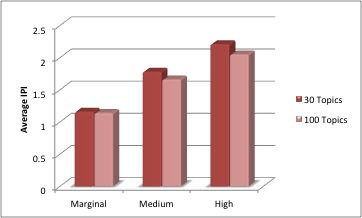
\includegraphics[scale=0.75]{IPIChart}
\end{center}
%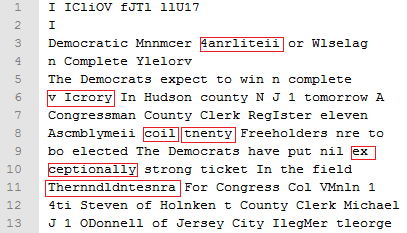
\includegraphics[scale=0.80]{ocr}
\caption{Comparison of the Average IPI for two ranked lists $L_1$ and $L_2$ using $30$ and $100$ topics respectively.}
\label{figure:IPI}
\end{figure*}

\subsection{An alternative approach for detecting influential persons}
\label{influential:BAMIC}
A heuristics based approach for finding influential persons has been discussed in the previous section. An alternative approach involving clustering can also be used for detection of influential persons.
 One such multiple instance clustering algorithm is suggested in \cite{zhang2009multi}.  They suggest an algorithm called BAMIC which can be applied to our problem as well. The multiple instance clustering problem considers clustering objects that consist of sets of instances for clustering rather than single instance clustering. According to the BAMIC algorithm, a set of instances is represented by a bag object and k-medoids algorithm is used to cluster those bags. The k-medoids algorithm is adapted to use average Hausdorff distance to measure the similarity between instances of different bags. It averages the distance between each instance in one bag and its nearest instance in the other bag and partitions dataset into k disjoint groups each containing a set of bags. BAMIC is applied to MUSK 1 and MUSK 2 datasets available publically\footnote{https://archive.ics.uci.edu/ml/datasets.html} which consist of 92 bags with 476 instances and 102 bags with 6598 instances, respectively and is used to test whether molecules are qualified to be used in a drug or not.
 This approach can be used to detect influential persons in our problem by clustering person entities into ``influential" or ``non-influential"  considering each person entity of our people gazetteer as a bag with articles of their occurrence as the instances for each bag. 
The parameters used for calculating DI in the previous section: NDL,NTF and NSIM can be used as features associated with each article instance in a bag.
Such a method can avoid choosing of parameter weights, biasing of results with respect to any specific parameter and decide which article plays a role in determining whether a person is influential or not. 
We tried to work with the open source version of the BAMIC algorithm to compare its results with the heuristic based approach suggested in this paper. But the clustering algorithm, due to its high complexity and the amount of data we worked with, the algorithm takes a very long time to give the results. Our dataset consisted of roughly 40000 person named entities on which multiple instance clustering was required and according to the estimation, it will take around 200 days to get the clusters of influential and influential persons.  Due to unavailability of such a long time frame, we do not present the results of comparison between the two approaches for detection of influential persons. Since BAMIC has been used for smaller datasets in earlier studies, we believe if the BAMIC algorithm can be scaled for larger datasets, it can be applied to our scenario easily.
